\documentclass[12pt]{article}
\usepackage[utf8x]{inputenc}
\usepackage[a4paper, nohead, dvips, left=30mm, right=20mm, top=20mm, bottom=20mm]{geometry}
\usepackage[english, russian]{babel}
\usepackage[T1, T2A]{fontenc}
\usepackage{amsthm}
\usepackage{amssymb}
\usepackage{amsmath}
\usepackage{graphicx}
\usepackage{subfigure}
\usepackage{float}
\usepackage{array}
\usepackage[ruled]{algorithm}
\usepackage{algorithmic}
\usepackage{ulem}
\usepackage[usenames, dvipsnames]{color}

\graphicspath{{../figures/eps/bw/}}

\theoremstyle{plain}
\newtheorem{theorem}{Теорема}
\newtheorem{lemma}{Лемма}
\theoremstyle{definition}
\newtheorem{definition}{Определение}

\def\figureref#1{Рис.\,\protect\ref{#1}}
\def\eqref#1{(\protect\ref{#1}\protect)}

\def\RC{\hbox{root-code}}
\def\RCD{\hbox{root-code-decomp}}


\begin{document}
	\Russian

	\newpage
	\section{Неальтернированные $k$-танглы}\label{section:non-alternating}

		Задача перечисления произвольных узлов, зацеплений и, соответственно, $k$-танглов является гораздо более сложной, чем аналогичная
		для альтернированного случая, и все известные на данный момент общие алгоритмы неприменимы из-за непрактичного времени работы. Даже
		для узлов самая большая на данный момент таблица~\cite{HosteThistlethwaiteWeeks1998} построена скорее с помощью ad hoc приемов и
		аккуратного программирования, а не какого-то общего алгоритма. Связано это с тем, что, хотя движения
		Рейдемейстера (см.~\figureref{figure:reidemeister-moves}) позволяют из любой диаграммы зацепления или $k$-тангла получить любую другую
		возможную его диаграмму, но в процессе преобразования может произойти увеличение числа перекрестков. Некоторые оценки на общее
		число движений известны~\cite{HassLagarias2001, Hayashi2005}, но полный перебор по-прежнему остается слишком трудоемким.

		\begin{figure}[ht]
			$$
			\def\pica#1{\raise-4mm\hbox{\protect\includegraphics[origin=c]{reidemeister-#1.eps}}}
			\pica{11}\ \backsimeq\ \pica{12}\qquad
			\pica{21}\ \backsimeq\ \pica{22}\qquad
			\pica{31}\ \backsimeq\ \pica{32}
			$$
			\caption{\footnotesize Движения Рейдемейстера.\label{figure:reidemeister-moves}}
		\end{figure}

		Как следствие, мы так просто уже не можем по диаграмме сказать, является ли она минимальной по числу перекрестков, а нашей задачей
		при перечислении является как раз нахождение для каждого $k$-тангла одной из его минимальных диаграмм. Более того, даже зная одну
		из минимальных диаграмм $k$-тангла, мы не можем просто узнать все остальные его минимальные диаграммы, поскольку какого-то набора
		движений, позволяющих получать друг из друга все возможные минимальные диаграммы, на данный момент неизвестно.

		Подобно использованному для узлов в~\cite{HosteThistlethwaiteWeeks1998}, наш метод перечисления произвольных $k$-танглов
		также состоит из трех шагов: генерирования некоторого множества диаграмм с перекрестками, удаления из полученного множества
		дубликатов c помощью движений Рейдемейстера и некоторого набора более сложных преобразований (которые, разумеется, представляются в
		виде нескольких последовательных движений Рейдемейстера, но значительно облегчают нам задачу) и, наконец, анализа получившихся
		диаграмм с помощью топологических инвариантов.

		Следующие три параграфа описывают три этих этапа соответственно. Затем следуют некоторые результаты с замечаниями.

	\subsection{Генерация диаграмм}

		Первым шагом к перечислению k-танглов будет перечисление всех возможных их простых связных диаграмм с точностью до поворотов, отражений
		и замены знаков всех перекрестков. Также нам хотелось бы избавится от диаграмм, которые немедленно упрощаются вторым движением
		Рейдемейстера (диаграмм, упрощающихся первым движением Рейдемейстера не будет, благодаря простоте). Для этого мы используем
		базирующееся на общей идее~\cite{McKay1998} обобщение алгоритма генерации проекций, описанного в \cite{BogdanovMeshkovOmelchenkoPetrov2011}.

		Для примера количества таких диаграмм с не более, чем 10 перекрестками, приведены в Таблице~\ref{table:tangle-diagrams}.

		\begin{table}[ht]
			\caption{Количество диаграмм $k$-танглов с $n$ перекрестками\label{table:tangle-diagrams}}
			\centering
			\begin{tabular}{|c||r|r|r|r|r|r|r|r|r|r|}
			\hline
			$k$\textbackslash $n$
			    & 1 & 2 &  3 &   4 &   5 &       6 &        7 &           8 &            9 &            10 \\
			\hline\hline
			2   & 1 & 1 &  3 &  14 &  76 &     486 &   3\,544 &     28\,357 &     239\,061 &   2\,094\,320 \\
			3   & . & 2 &  4 &  25 & 148 &  1\,146 &   9\,036 &     76\,696 &     670\,368 &   6\,027\,768 \\
			4   & . & . &  6 &  33 & 258 &  2\,125 &  18\,537 &    165\,895 &  1\,518\,645 &  14\,133\,545 \\
			5   & . & . &  . &  32 & 290 &  3\,086 &  30\,276 &    298\,392 &  2\,919\,788 &  28\,649\,272 \\
			6   & . & . &  . &   . & 206 &  3\,081 &  38\,515 &    435\,907 &  4\,726\,468 &  50\,026\,435 \\
			7   & . & . &  . &   . &   . &  1\,718 &  33\,645 &    490\,784 &  6\,223\,320 &  73\,693\,696 \\
			8   & . & . &  . &   . &   . &       . &  15\,722 &    380\,276 &  6\,298\,284 &  88\,352\,732 \\
			9   & . & . &  . &   . &   . &       . &        . &    154\,656 &  4\,376\,155 &  81\,234\,008 \\
			10  & . & . &  . &   . &   . &       . &        . &           . &  1\,580\,929 &  51\,154\,784 \\
			11  & . & . &  . &   . &   . &       . &        . &           . &            . &  16\,656\,936 \\
			\hline
			all & 1 & 3 & 13 & 104 & 978 & 11\,642 & 149\,275 & 2\,030\,963 & 28\,553\,018 & 412\,023\,496 \\
			\hline
			\end{tabular}
		\end{table}

	\subsection{Движения}

		После того, как мы научились получать диаграммы $k$-танглов, будем действовать следующим образом: поддерживать с помощью
		систем непересекающихся множеств~\cite{CormenLeisersonRivestStein2009, Sedgewick1983} на них соотношение эквивалентности, для
		каждой из диаграмм объявляя эквивалентными ей те, которые могут быть получены из нее применением одного из движений, о которых
		речь пойдет ниже, и затем, если возможно, то уменьшением числа перекрестков с помощью первого и второго движений Рейдемейстера
		жадным образом (легко показать, что результат такой жадной редукции не зависит от выбора порядка применяемых движений).

		\begin{figure}[ht]
			\centering
			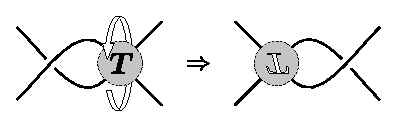
\includegraphics{c/flype.eps}
			\caption{\footnotesize Flype.\label{figure:flype}}
		\end{figure}

		Хотя такая схема приводит к большому расходу памяти и не может быть использована в действительно объемном перечислении, но это
		в данном случае не является проблемой и даже дает некоторые преимущества, так как, во-первых, лимитирующим фактором перечисления,
		как будет понятно из дальнейшего, является сила используемых для доказательства различности полученных классов эквивалентности
		топологических инвариантов, и, во-вторых, подход позволяет ``заглянуть вперед'' по количеству перекрестков и обнаружить пары
		эквивалентных диаграмм, которые не объединились с помощью только набора движений, что может служить подсказками для изобретения
		новых более сложных движений.

		\begin{figure}[ht]
			\centering
			$$
			{\raise-4mm\hbox{\protect\includegraphics{pass-1.eps}}}
			\qquad
			{\raise-5mm\hbox{\protect\includegraphics{pass-2.eps}}}
			$$
			\caption{\footnotesize Pass.\label{figure:pass}}
		\end{figure}

		В качестве собственно движений мы будем использовать третье преобразование Рейдемейстера, flype (см.~\figureref{figure:flype}), а также
		pass, являющийся обобщением третьего преобразования Рейдемейстера --- давно известное движение (первые составители таблиц узлов
		предполагали, что пары из flype и pass достаточно, чтобы показать эквивалентность любой пары минимальных диаграмм любого узла).
		Следует, однако, заметить, что в, отличие от узлов, для $k$-танглов существует два возможных варианта движения pass
		(см.~\figureref{figure:pass}).

	\subsection{Инварианты}

		Следующим шагом к перечислению неальтернированных $k$-танглов является доказательство того, что полученные на предыдущем шаге
		классы эквивалентности соответствуют действительно неэквивалентным $k$-танглам. Для этого мы используем модификацию полинома
		Джонса~\cite{Jones2005}, заключающуюся в сведении диаграммы всеми возможными способами с помощью скейн-соотношений:

		$$
		\begin{aligned}
			& \langle \ell \rangle = a\langle \ell_1 \rangle + \frac{1}{a} \langle {\ell_2} \rangle \\
			& \langle {\ell{\textstyle{}\bigcup{}}\bigcirc} \rangle = -\left( a^2 + \frac{1}{a^2} \right) \langle \ell \rangle \\
			& 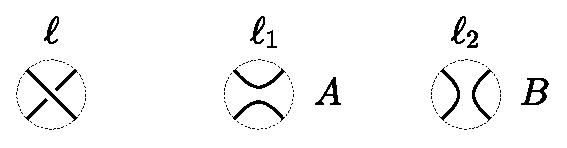
\includegraphics[scale=0.5]{c/kauffman-skein-definition.eps}
		\end{aligned}
		$$

		к некоторому множеству диаграмм без перекрестков (см.~\figureref{figure:jones-example}). Так как любое применение скейн-соотношения
		уменьшает количество перекрестков на единицу, любая диаграмма $k$-тангла может быть сведена к набору хордовых диаграмм без пересечений,
		имеющих взаимно однозначное соответствие с правильными скобочными последовательностями длины $2 k$. Таким образом можно получить
		топологический инвариант $k$-танглов, принимающий значения в модуле над полиномами Лорана с базисом из правильных скобочных
		последовательностей. Далее мы избавимя от поворотов и отражений, введя на полученных значениях лексикографический порядок и
		минимизируя относительно него.

		\begin{figure}[ht]
			\centering
			$$
			\def\pica#1{\raise-5mm\hbox{\protect\includegraphics[origin=c]{tangle-jones-skein-example-#1.eps}}}
			\pica{1} = a^3 \pica{2} + a \pica{3} + (a - a^{-3}) \pica{4} + (a^{-1} - a^{-5}) \pica{5}
			$$
			\caption{\footnotesize Пример применения скейн-соотношений.\label{figure:jones-example}}
		\end{figure}

		Полученный инвариант сам по себе дает коллизии уже для диаграмм с пятью перекрестками, то есть работает значительно хуже, чем полином
		Джонса для узлов и зацеплений. Чтобы получить лучший инвариант, мы применим следующее преобразование над диаграммой: раздвоим каждую
		нить и при необходимости добавим дополнительные перекрестки так, чтобы каждая пара новых нитей имела нулевое число зацепления
		(см.~\figureref{figure:tangle-doubling-example}), и будем вычислять полином Джонса уже от такой модифицированной диаграммы. Такая
		конструкция является более сильным инвариантом, однако все же не позволяет различать диаграммы, отличающиеся мутацией.

		\begin{figure}[ht]
			\centering
			$$
			\def\pica#1{\raise-13mm\hbox{\protect\includegraphics[origin=c,scale=0.3]{tangle-doubling-example-#1.eps}}}
			\pica{1}\ \Rightarrow\ \pica{2}
			$$
			\caption{\footnotesize Пример удвоения $k$-тангла.\label{figure:tangle-doubling-example}}
		\end{figure}

	\subsection{Результаты}

		\begin{table}[ht]
			\caption{Количество $k$-танглов с $n$ перекрестками.\label{table:non-alternating-tangles}}
			\centering
			\let\ul=\underline
			\begin{tabular}{|c||r|r|r|r|r|r|r|r|}
			\hline
			$k$\textbackslash $n$
			    & 1 & 2 &  3 &  4 &   5 &      6 &        7 &           8 \\
			\hline\hline
			2   & 1 & 1 &  2 &  6 &  15 &     47 &      156 &    \ul{589} \\
			3   & . & 2 &  4 & 15 &  48 &    201 & \ul{811} & \ul{3\,755} \\
			4   & . & . &  6 & 30 & 154 &    762 &   3\,796 &     19\,468 \\
			5   & . & . &  . & 32 & 258 & 1\,916 &  11\,931 &     71\,943 \\
			6   & . & . &  . &  . & 206 & 2\,717 &  24\,735 &    186\,790 \\
			7   & . & . &  . &  . &   . & 1\,718 &  29\,572 &    323\,781 \\
			8   & . & . &  . &  . &   . &      . &  15\,722 &    333\,764 \\
			9   & . & . &  . &  . &   . &      . &        . &    154\,656 \\
			\hline
			all & 1 & 3 & 12 & 83 & 681 & 7\,361 &  86\,724 & 1\,094\,746 \\
			\hline
			\end{tabular}
		\end{table}

		\begin{figure}[ht]
			\centering
			\includegraphics[scale=0.8]{nonalternating-tangles-1.eps}
			\caption{\footnotesize Неальтернированные $k$-танглы до 4-х перекрестков.\label{figure:nonalternating-tangles-4}}
		\end{figure}

		\begin{figure}[ht]
			\centering
			\includegraphics[scale=0.8]{nonalternating-tangles-2.eps}
			\caption{\footnotesize Некоторые другие неальтернированные $k$-танглы.\label{figure:nonalternating-tangles-rest}}
		\end{figure}

		\begin{table}[ht]
			\caption{Количество слабо эквивалентных $k$-танглов с $n$ перекрестками.\label{table:weak-tangles}}
			\centering
			\begin{tabular}{|c||r|r|r|r|r|}
			\hline
			$k$\textbackslash $n$
			    & 4 & 5 & 6 &  7 &   8 \\
			\hline\hline
			2   & 1 & 2 & 8 & 29 & 132 \\
			3   & . & . & 1 &  2 &  14 \\
			4   & . & . & . &  . &  16 \\
			\hline
			all & 1 & 2 & 9 & 31 & 162 \\
			\hline
			\end{tabular}
		\end{table}

		\begin{figure}[ht]
			\centering
			\includegraphics[scale=0.8]{nonalternating-tangles-3.eps}
			\caption{\footnotesize $k$-танглы до 7 перекрестков с точностью до слабой эквивалентности.\label{figure:weak-tangles-7}}
		\end{figure}

		Количества $k$-танглов до 8 перекрестков приведены в Таблице~\ref{table:non-alternating-tangles}. Все числа, кроме подчеркнутых,
		соответствуют спискам диаграммам, про которые доказанно с помощью инвариантов отсутствие в них дубликатов. Среди остальных
		диаграмм, соответствующих подчеркнутым числам, встречаются пары и четверки, дающие одинаковые инварианты
		(см. \figureref{figure:nonalt-collisions-8-2}, \figureref{figure:nonalt-collisions-7-3}, \figureref{figure:nonalt-collisions-8-3}).

		Изображения некоторых неальтернированных $k$-танглов приведены на \figureref{figure:nonalternating-tangles-4} и
		\figureref{figure:nonalternating-tangles-rest}.

		Также мы пытались повторить результаты~\cite{KanenobuSaitoSatoh2003}, где были вручную перечислены $2$-танглы не более чем
		с 7 перекрестками с точностью до слабой эквивалентности. Получившиеся количества и некоторые диаграммы приведены в
		Таблице~\ref{table:weak-tangles} и на~\figureref{figure:weak-tangles-7} соответственно. Следует отметить, что для 7
		перекрестков у нас получилось на один $2$-тангл больше, чем в~\cite{KanenobuSaitoSatoh2003}.
%		``Лишним'' является предпоследний
%		в первом ряду $2$-тангл из соответствующей группы на~\figureref{figure:weak-tangles-7}.

		Исходный код программы на \texttt{Haskell}, используемой нами при перечислении, можно найти в открытом репозитории по
		адресу \texttt{https://github.com/mishun/tangles}.

		\begin{figure}[ht]
			\centering
			\includegraphics[scale=1]{nonalt-collisions-jones-double-jones-1.eps}
			\caption{\footnotesize Коллизии для 2-танглов с 8 перекрестками.\label{figure:nonalt-collisions-8-2}}
		\end{figure}

		\begin{figure}[ht]
			\centering
			\includegraphics[scale=1]{nonalt-collisions-jones-double-jones-2.eps}
			\caption{\footnotesize Коллизии для 3-танглов с 7 перекрестками.\label{figure:nonalt-collisions-7-3}}
		\end{figure}

		\begin{figure}[ht]
			\centering
			\includegraphics[scale=0.75]{nonalt-collisions-jones-double-jones-3.eps}
			\caption{\footnotesize Коллизии для 3-танглов с 8 перекрестками.\label{figure:nonalt-collisions-8-3}}
		\end{figure}

	\newpage
	\begin{thebibliography}{88}

		\bibitem{BogdanovMeshkovOmelchenkoPetrov2011}
		{\em Bogdanov~A., Meshkov~V., Omelchenko~A., Petrov~M.}
		Classification of $k$-tangle projections using cascade representation.
		Journal of Knot Theory and Its Ramifications, to appear.
		e-print: \texttt{arXiv:0712.3859v2}

		\bibitem{Conway1970}
		{\em Conway~J.}
		An enumeration of knots and links, and some of their algebraic properties.
		Computational Problems in Abstract Algebra (John Leech, ed.), Pergamon Press, Oxford
		and New York, 1969, 329--358.

		\bibitem{CormenLeisersonRivestStein2009}
		{\em Cormen~T., Leiserson~C., Rivest~R., Stein~C.}
		Introduction to Algorithms (3rd ed.).
		MIT Press., 2009.

		\bibitem{Cromwell2004}
		{\em Cromwell~P.}
		Knots and links.
		Cambridge university press, 2004, 350\,с.

		\bibitem{Jones2005}
		{\em Jones~V.}
		The Jones Polynomial.
		\texttt{http://www.math.berkeley.edu/\textasciitilde vfr/jones.pdf}

		\bibitem{HassLagarias2001}
		{\em Hass~J., Lagarias~J.}
		The number of Reidemeister moves needed for unknotting.
		J. Amer. Math. Soc. 14 (2001), no. 2, 399--428

		\bibitem{Hayashi2005}
		{\em Hayashi~C.}
		The number of Reidemeister moves for splitting a link.
		Math. Ann., 2005, Vol.\,332, {\bf 2}, 239--252.

		\bibitem{HosteThistlethwaiteWeeks1998}
		{\em Hoste~J., Thistlethwaite~M., Weeks~J.}
		The first 1,701,936 knots.
		Math. Intelligencer, 1998, Vol.\,20, {\bf 4}, 33--48 (1998).

		\bibitem{KanenobuSaitoSatoh2003}
		{\em Kanenobu~T., Saito~H., and Satoh~S.}
		Tangles with up to seven crossings.
		Interdisciplinary Information Sciences, 2003, Vol.\,9, {\bf 1}, 127--140.

		\bibitem{Kauffman1987}
		{\em Kauffman~L.~H.}
		State Models and the Jones Polynomial.
		Topology, 1987, {\bf 26}, 395--407.

		\bibitem{KauffmanLambropoulou2004}
		{\em Kauffman~L., Lambropoulou~S.}
		On the classification of rational tangles.
		Advances in Applied Mathematics, 2004, {\bf 2}, 199--237.
		e-print:~\texttt{arXiv:math/0311499v2}.

		\bibitem{McKay1998}
		{\em McKay~B.~D.}
		Isomorph-free exhaustive generation.
		J. Algorithms, 1998, {\bf 26}, 306--324.

		\bibitem{MenascoThistlethwaite1991}
		{\em Menasco~W., Thistlethwaite~M.}
		The Tait Flyping Conjecture.
		Bull. Amer. Math. Soc., 1991, {\bf 25}, 403--412.

		\bibitem{MenascoThistlethwaite1993}
		{\em Menasco~W., Thistlethwaite~M.}
		The Classification of Alternating Links.
		Ann. Math., 1993, {\bf 138}, 113--171.

		\bibitem{Murasugi1987_1}
		{\em Murasugi~K.}
		The Jones Polynomial and Classical Conjectures in Knot Theory.
		Topology, 1987, {\bf 26}, 187--194.

		\bibitem{Murasugi1987_2}
		{\em Murasugi~K.}
		Jones Polynomials and Classical Conjectures in Knot Theory II.
		Math. Proc. Cambridge Philos. Soc., 1987, {\bf 102}, 317--318.

		\bibitem{RankinSchermannSmith2002_1}
		{\em Rankin~S., Schermann~J., Smith~O.}
		Enumerating the prime alternating knots, Part I,
		Journal of Knot Theory and Its Ramifications, 2004, Vol.\,13, {\bf 1}, 57--100.
		e-print:~\texttt{arXiv:math/0211346}

		\bibitem{RankinSchermannSmith2002_2}
		{\em Rankin~S., Schermann~J., Smith~O.}
		Enumerating the prime alternating knots, Part II,
		Journal of Knot Theory and Its Ramifications, 2004, Vol.\,13, {\bf 1}, 101--149.
		e-print:~\texttt{arXiv:math/0211348}

		\bibitem{RankinSmith2002}
		{\em Rankin~S., Smith~O.}
		Enumerating the Prime Alternating Links.
		Journal of Knot Theory and Its Ramifications, 2004, Vol.\,13, {\bf 1}, 151--173.
		e-print:~\texttt{arXiv:math/0211451}

		\bibitem{Sedgewick1983}
		{\em Sedgewick~R.}
		Algorithms (1st ed.).
		Addison-Wesley, 1983.

		\bibitem{SundbergThistlethwaite1998}
		{\em Sundberg~C., Thistlethwaite~M.}
		The Rate of Growth of the Number of Prime Alternating Links and Tangles.
		Pacific Journal of Mathematics, 1998, Vol.\,182, {\bf 2}, 329--358.

		\bibitem{Tait1900}
		{\em Tait~P.~G.}
		On Knots I, II, III.
		Scientific Papers.
		London: Cambridge University Press, 1900, Vol.\,1, 273--347.

		\bibitem{Thistlethwaite1987}
		{\em Thistlethwaite~M.}
		A Spanning Tree Expansion of the Jones Polynomial.
		Topology, 1987, {\bf 26}, 297--309. 

		\bibitem{Thistlethwaite1988}
		{\em Thistlethwaite~M.}
		Kauffman's Polynomial and Alternating Links.
		Topology, 1988, {\bf 27}, 311--318.

		\bibitem{JustinZuber2003}
		{\em Zinn-Justin~P., Zuber~J.}
		Matrix integrals and the generation and counting of virtual tangles and links.
		Journal of Knot Theory and Its Ramification, 2004, Vol.\,13, {\bf 2}, 325--356.
		e-print:~\texttt{arXiv:math-ph/0303049}.

	\end{thebibliography}
\end{document}
